%----------------------------------------------------------------------------------------
%	PACKAGES AND OTHER DOCUMENT CONFIGURATIONS
%----------------------------------------------------------------------------------------

\documentclass[12pt]{article}
\usepackage[danish]{babel}
\usepackage[numbered,final]{mcode}
\usepackage[utf8x]{inputenc}
\usepackage{amsmath}
\usepackage{graphicx}
\usepackage[colorinlistoftodos]{todonotes}
\usepackage[toc,page]{appendix}
%\usepackage{float}
\usepackage{floatrow} % used for adding "Source" to pictures
\usepackage{hyperref} % used for hyperlinks
\usepackage[all]{hypcap}
\usepackage{bm} % used for bold inline matj
\usepackage{lipsum} % used for lorem lipsum
\usepackage[final]{pdfpages} % used for including PDF's
\usepackage{geometry}
\usepackage{listingsutf8}
\usepackage{listings}
\usepackage{color} %red, green, blue, yellow, cyan, magenta, black, white
\definecolor{mygreen}{RGB}{28,172,0} % color values Red, Green, Blue
\definecolor{mylilas}{RGB}{170,55,241}

\hypersetup{colorlinks=true, linkcolor=black}

% Page margins
\geometry{verbose,tmargin=1in,bmargin=1in,lmargin=1in,rmargin=1in,headsep=0.35in}


\begin{document}
	
	\begin{titlepage}
		
		
		
		\newcommand{\HRule}{\rule{\linewidth}{0.5mm}} % Defines a new command for the horizontal lines, change thickness here
		\setlength{\topmargin}{0in}
		\centering % Center everything on the page
		
		%----------------------------------------------------------------------------------------
		%	HEADING SECTIONS
		%----------------------------------------------------------------------------------------
		\textsc{\LARGE Aarhus universitet}\\[1.5cm] % Name of your university/college
		\textsc{\Large Indlejret Signalbehandling}\\[0.5cm] % Major heading such as course name
		\textsc{\large 6. Semester}\\[0.5cm] % Minor heading such as course title
		
		%----------------------------------------------------------------------------------------
		%	TITLE SECTION
		%----------------------------------------------------------------------------------------
		
		\HRule \\[0.4cm]
		{ \huge \bfseries ISB projekt}\\ % Title of your document
		\HRule \\[1cm]
		
		%----------------------------------------------------------------------------------------
		%	AUTHOR SECTION
		%----------------------------------------------------------------------------------------
		
		\begin{minipage}{0.4\textwidth}
			\begin{flushleft} \large
				\emph{Gruppemedlemmer:}\\
				Søren Landgrebe \\
				Stinus Lykke Skovgaard \\
			\end{flushleft}
		\end{minipage}
		~
		\begin{minipage}{0.4\textwidth}
			\begin{flushright} \large
				\emph{Studienr:} \\
				201508295\\
				201401682\
			\end{flushright}
		\end{minipage}\\[5cm]
		
		%----------------------------------------------------------------------------------------
		%	LOGO SECTION
		%----------------------------------------------------------------------------------------
		
		
\includegraphics[scale=0.5]{Img/logo.jpg}\\[1cm]
		
		%----------------------------------------------------------------------------------------
		%	DATE SECTION
		%----------------------------------------------------------------------------------------
		
		{\large \today}\\[0.5cm] % Date, change the \today to a set date if you want to be precise
		
		
		\vfill % Fill the rest of the page with whitespace
		
	\end{titlepage}
	
\newpage
\tableofcontents
\newpage
\listoffigures
\newpage

\hypersetup{linkcolor=blue}

\label{sec:MyMultiply_funktion}
%!TEX root = ../../Main.tex
\graphicspath{{Chapters/Indledning/}}
%-------------------------------------------------------------------------------

\chapter{Indledning}
\section{Indledning}
Under optagelse til et live madprogram, sker det ofte at værten skal bruge en blender/foodprocesser. Dette betyder at værten ikke kan kommunikere med seerne mens blenderen/foodprocesseren kører. Denne problematik vil Noise Suppression System (NSS) kunne afhjælpe. Gennem en digital signal prossesering (DSP), vil vi dæmpe støjsignalet fra en køkkenmaskine dynamisk i realtid. Systemet består af to mikrofoner, et placeres tæt på støjen, et andet tæt på værten. De to mikrofoner fungere som input til vores system (Blackfin), hvor procceseringen og filtreringen foregår. Efter proceseringen bliver produktet afspillet på en højtaler, som erstatning for højtaleren fra et tv-apperat. Et overblik over systemet kan ses på figur \ref{fig:konceptbillede}

\begin{figure}[H]
	\centering
	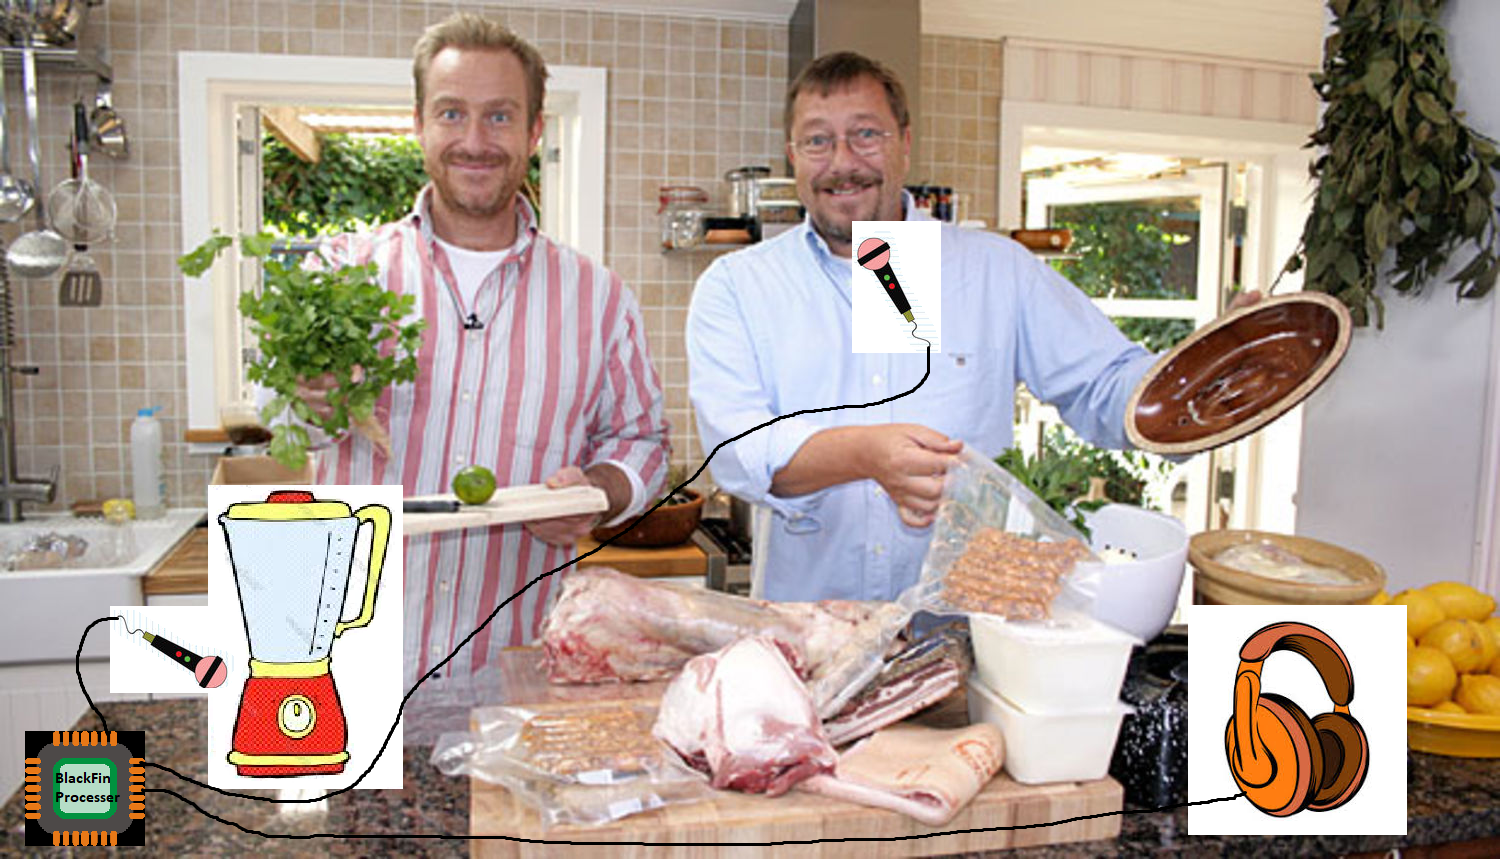
\includegraphics[width = 400pt]{Img/Konceptbillede}
	\caption{Konceptbillede for NSS}
	\label{fig:konceptbillede}
\end{figure}

Med udgangspunkt i brugerens behov vil der blive opstillet en række brugsscenarier, der beskriver brugerens interaktion med systemet. Disse scenarier vil sammen med en række veldefinerede krav og afgrænsninger, danne grundlaget for designet af alle dele af systemet.  \\ 

\newpage


	%!TEX root = ../../Main.tex
\graphicspath{{Chapters/Krav/}}
%-------------------------------------------------------------------------------


\section{Krav}
I dette afsnit beskrives kravene til hvilken funktionalitet systemet har. 


I samarbejde med vejleder er der opstillet en række krav.
\begin{itemize}
\item Systemets skal kunne filtrere en støj fra et lydsignal, som indeholder et tale signal overlappet af et støjsignal.
\item Brugeren skal manuelt kunne tænde og slukke for filtreringen.
\item Output lydsignalet skal feedes til en højtaler som afspiller lyden fra mikrofonen. 
\end{itemize}

Kravene er bygget op gennem use cases, som beskriver systemets funktionelle krav, samt en liste over alle ikke-funktionelle krav for systemet. Først vises aktørbeskrivelserne
med tilhørende aktørkontekst diagram. Herefter vises use cases for systemet. Der er udfærdiget to use cases
der tilsammen beskriver funktionaliteten af systemet. I use case afsnittet vises der også et use case diagram
med alle use cases og hvordan aktørerne interagerer med dem. Til sidst gives et kort overblik over ikke funktionelle krav.

\section{Aktørbeskrivelse}

\begin{figure}[H]
	\centering
	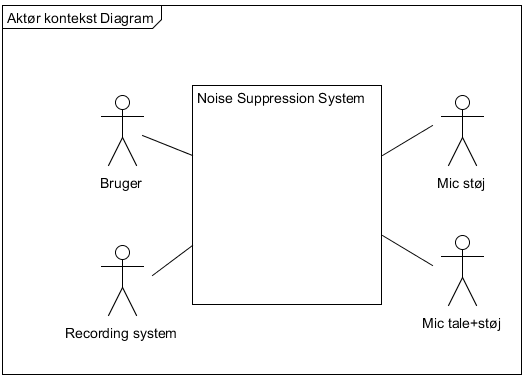
\includegraphics[width = 200 pt]{Img/Aktoer_Kontekst.png}
	\caption{Aktør Kontekst diagram}
	\label{fig:Aktoer Kontekst diagram}
\end{figure}

På figur \ref{fig:Aktoer Kontekst diagram} ses aktør kontekst diagrammet som beskriver sammenhængen mellem aktørene og det system de interagere med. Aktørene er som følger: \\*
\textbf{Primær}\\
\textbf{Bruger:} Den aktør der interagerer med systemet og vælger den ønskede funktionalitet \\
\textbf{Recording system:} Den aktør der modtager det enedelige produkt\\
\textbf{Sekundær}\\
\textbf{Mic støj:} Et input til det samlede system\\
\textbf{Mic tale+støj:} Et input til det samlede system \\

\section{Use case beskrivelse}

\begin{figure}[H]
	\centering
	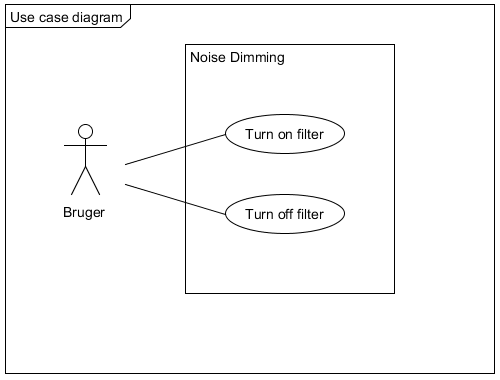
\includegraphics[width = 300 pt]{Img/Usecase_Diagram.png}
	\caption{Usecase diagram}
	\label{fig:Usecase diagram}
\end{figure}

På figur \ref{fig:Usecase diagram} ses usecase diagrammet som beskriver sammenhængen mellem aktørerne og de forskellige funktionaliteter der findes for systemet.

\subsubsection{UC 1 - Turn on filter}

Brugeren trykker på SW1 og filteret aktiveres. 


\subsubsection{UC 2 - Turn off filter}

Brugeren trykker på SW1 og filteret deaktiveres. 

\subsubsection{UC 3 - Filter aktiv}

Recording system modtager det filtrede lyd, hvis prækonditionen UC 1  er udført. 

\newpage
\section{Ikke-funktionelle krav}
Kravene er delt op i tre underkategorier. Krav der relaterer til problemet. krav der relaterer til DSP platform og algoritme. Til sidst er der en kategori der beskriver kravene til systemet på baggrund af de to første kategorier.
\begin{enumerate}
	
	\subsection{Problemrelateret krav}
	\item R1: Systemet skal have 2 mikrofoner og 1 højtaler
	
	\item R2: Filteret skal gøre brug af LMS algoritmen
	
	\item R3: Systemet skal kunne processerer lyd i frekvensbåndet 50-20000Hz. 
	
	\item R4: Systemet skal kunne dæmpe uønkset støj 30dB.
	
	\item R5: Systemet skal kunne dæmpe støj uden at dæmpe ønsket lydsignal.
	
	\item R6: Systemet burde have en latency under 30ms.
	
	\item R7: Systemet burde have et dynamikområde på min 80dB
	
	\subsection{System og algoritme krav}
	
	\item R8: Filter algoritmen skal implementeres med fixed point 
	
	\item R9: Filteret skal max bruge 10kByte memory
	
	\item R10: Filteret skal implementeres på Blackfin BF533
	
	\item R11: Filteret må max benytte 98\% DSP load

	\subsection{Afledte krav}
	
	\item DR1: DSP systemet skal kunne håndtere en samplingsrate på min 44100kHz(På baggrund af krav R3) 
	
	\item DR2: Filteret skal implementeres med 1.15 fixed point.(På baggrund af krav R7 og R8. Dette giver et dynamikområde på 96dB)
	
	\item DR3: Filter latency må max forsinkes 1280 samples(På baggrund af R6. (1/44100)*1280=30ms)
	
	\item Filteret må max bruge 13333 cycles af DSP processering for hver sample. (På baggrund af R10, R11 og DR1 (600MHz/44.1kHz)*90\%)
	
\end{enumerate}


\section{Acceptest}
Til hver use case er der lavet en tilhørende accepttest, der tjekker om use casen bliver gennemført korrekt. Udover de tre accepttests er der oprettet en accepttest af de ikke-funktionelle krav til systemet. Alle accepttests kan ses
i kravspecifikations dokumentation.

\begin{flushleft}
	
\end{flushleft}

	
	

\end{document}